\documentclass{article}
\usepackage[utf8]{inputenc}
\usepackage[spanish]{babel}
\usepackage{listingsutf8}
\usepackage{xcolor}
\usepackage{pdfpages}
\usepackage{geometry}
% to install algorithm2e pckg: sudo apt-get install texlive-science
\usepackage[ruled, vlined, nofillcomment]{algorithm2e}

\geometry{
    a4paper,
    margin=1.2in
}

\title{75.29 - Teoría de Algoritmos I: Trabajo Práctico n. 2}
\author{
    \\\\\\\\
    \Large{Equipo Q:}\\
    Lavandeira, Lucas (\texttt{\#98042})\\\texttt{}\\
    \\
    Rozanec, Matias (\texttt{\#97404})\\\texttt{rozanecm@gmail.com}\\
    \\
    Sbruzzi, José (\texttt{\#97452})\\\texttt{}\\
    \\\\\\\\\\\\\\
}
\date{14.mayo.2018}

\begin{document}
\maketitle
\begin{figure}[!htp]
    \centering
    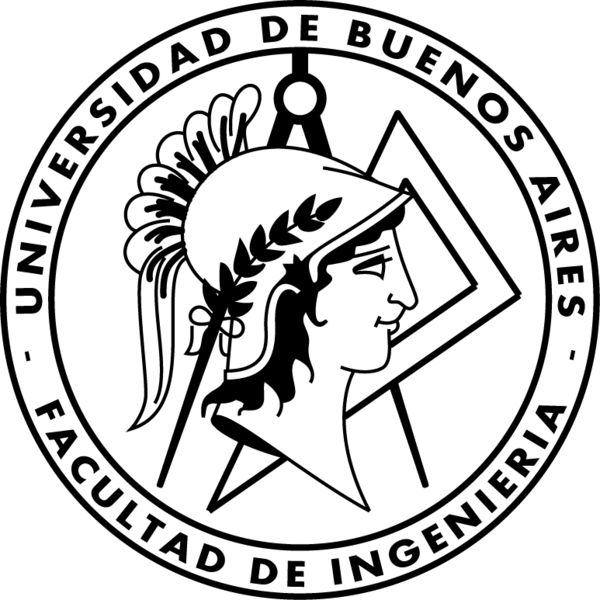
\includegraphics[scale=1]{res/fiuba_logo.png} 
\end{figure}
\begin{center}\normalsize{Facultad de Ingeniería, Universidad de Buenos Aires}\end{center}
\newpage

\tableofcontents
\newpage

% *** RESOLUCION ***
% Some settings for coding style
\lstset{
    basicstyle=\linespread{0.9}\ttfamily\footnotesize,
    frame=single,
    frameround=tttt,
    numbers=left,
    numberstyle=\tiny,
    linewidth=14cm,
    literate=
      {á}{{\'a}}1 {é}{{\'e}}1 {í}{{\'i}}1 {ó}{{\'o}}1 {ú}{{\'u}}1
      {Á}{{\'A}}1 {É}{{\'E}}1 {Í}{{\'I}}1 {Ó}{{\'O}}1 {Ú}{{\'U}}1
      {à}{{\`a}}1 {è}{{\`e}}1 {ì}{{\`i}}1 {ò}{{\`o}}1 {ù}{{\`u}}1
      {À}{{\`A}}1 {È}{{\'E}}1 {Ì}{{\`I}}1 {Ò}{{\`O}}1 {Ù}{{\`U}}1
      {ä}{{\"a}}1 {ë}{{\"e}}1 {ï}{{\"i}}1 {ö}{{\"o}}1 {ü}{{\"u}}1
      {Ä}{{\"A}}1 {Ë}{{\"E}}1 {Ï}{{\"I}}1 {Ö}{{\"O}}1 {Ü}{{\"U}}1
      {â}{{\^a}}1 {ê}{{\^e}}1 {î}{{\^i}}1 {ô}{{\^o}}1 {û}{{\^u}}1
      {Â}{{\^A}}1 {Ê}{{\^E}}1 {Î}{{\^I}}1 {Ô}{{\^O}}1 {Û}{{\^U}}1
      {œ}{{\oe}}1 {Œ}{{\OE}}1 {æ}{{\ae}}1 {Æ}{{\AE}}1 {ß}{{\ss}}1
      {ű}{{\H{u}}}1 {Ű}{{\H{U}}}1 {ő}{{\H{o}}}1 {Ő}{{\H{O}}}1
      {ç}{{\c c}}1 {Ç}{{\c C}}1 {ø}{{\o}}1 {å}{{\r a}}1 {Å}{{\r A}}1
      {€}{{\euro}}1 {£}{{\pounds}}1 {«}{{\guillemotleft}}1
      {»}{{\guillemotright}}1 {ñ}{{\~n}}1 {Ñ}{{\~N}}1 {¿}{{?`}}1
}
\part{Resolución}
\section{Parte 1: Spy vs Spy}
\section{Parte 2}
\subsection{Ejercicio 1}
\subsection{Ejercicio 2}
\subsection{Ejercicio 3}
Como primer paso, demostraremos que, dada una cantidad $n$ de cursos, si llamamos $m$ a la cantidad máxima de cursos superpuestos en cualquier instante de tiempo, la cantidad de aulas necesarias para realizar la asignación es $m$.\\

\textbf{Demostración}\par
Para demostrar esto, se plantearán las cotas superior e inferior, y se demostrará que ambas coinciden, siendo el valor de ambas: $m$.\\

\textbf{Cota inferior}\par
De haber $m$ cursos que se dictan al mismo tiempo, como no se pueden dictar cursos distintos en una misma aula en simultáneo, queda probado que como mínimo debe haber tantas aulas como cursos se dictan en simultáneo. Por lo tanto, es válido afirmar que $$Aulas\ necesarias \geq m$$\par
\textbf{Cota superior}\par
Para todo instante $t$ de tiempo habrá, según lo demostrado anteriormente, como mínimo $m$ aulas disponibles. Se puede comprobar rápidamente que para ningún $t$ se necesitarán más que $m$ aulas, dado que si dos cursos no se superponen temporalmente, no hay razón por la que no puedan compartir una misma aula. Además se está tratando el caso en que todas las aulas son iguales, lo que evita complicaciones más allá del análisis presentado.

Llegamos entonces a que $$Aulas\ necesarias \leq m$$
Queda así demostrado que $Aulas\ necesarias = m$
\subsubsection{Pseudocódigo}
\begin{algorithm}[H]
    \KwData{Horarios de inicio y finalización de cada uno de los $n$ cursos: $T_{inicio,j}$ y $T_{fin,j}$ denotan los tiempos de inicio y finalización del curso $j-$ésimo. Conjunto de todos los tiempos: $T_i, i\in (1, 2n)$}
    \KwResult{Menor cantidad de aulas necesarias para acomodar todos los cursos suponiendo que todas las aulas son iguales.}
    \BlankLine
    min time slice $\leftarrow \infty$\;
    min time $\leftarrow \infty$\;
    max time $\leftarrow 0$\;
    \ForEach{$T_i$}{
        \If{$(current\ min\ slice = |T_i - T_j|)<min\_aulas, i\neq j$}{
            min time slice := current min\;
        }
        \If{$T_i < $ min time}{
            min time := $T_i$\;
        }
        \If{$T_i > $ max time}{
            max time := $T_i$\;
        }
    }
    \BlankLine
    current time := min time\;
    max superpositions := 0\;
    \While{min time $<$ max time}{
        current num of superpositions := 0\;
        \ForEach{$T_{inicio,j}, T_{fin,j}$}{
            \If{$T_{inicio,j} \geq$ current time slice AND $> T_{fin,j}$}{
                ++current num of superpositions\;
            }
        }
        \If{current num of superpositions $>$ max superpositions}{
            max superpositions := current num of superpositions\;
        }
        current time += min time slice\;
    }
\caption{Pseudo código que resuelve el problema.}
\end{algorithm}
\end{document}
